\begin{frame}\frametitle{Interesting alternative: Unscented Kalman Filter (UKF)}
The goal stays the same: to estimate the state $\vect{X}(k)$: mean ($\hat{X}$) and covariance ($P$). %Framework is similar: Nonlinear filter that does \textit{prediction \& correction}, uses Bayesian approach. \\
\vspace{-5pt}
\begin{columns}
	\column{.45\textwidth}
	\begin{block}{e.g. Mapping from Polar to Cartesian coordinates}
	\centering
	\begin{figure}
	\subfigure[{\scriptsize polar coord.}]{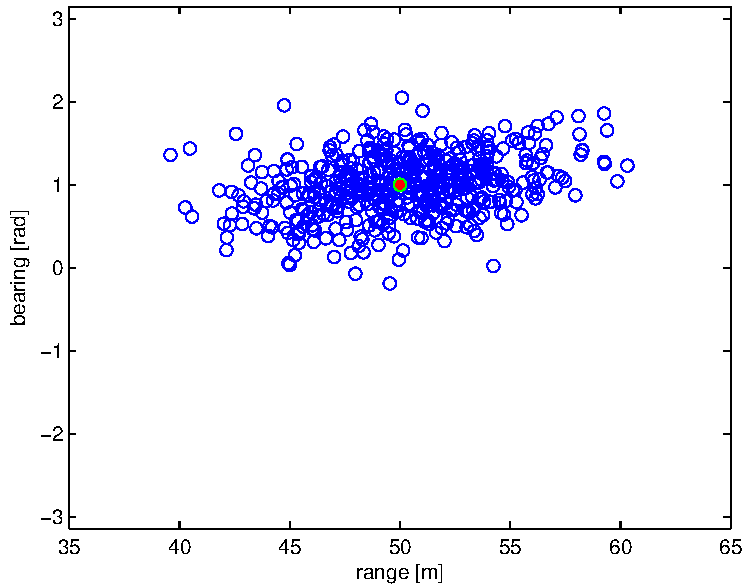
\includegraphics[width=0.45\linewidth]{fig/orig.pdf}}
	\subfigure[{\scriptsize $\hat{X}, P$ (EKF)}]{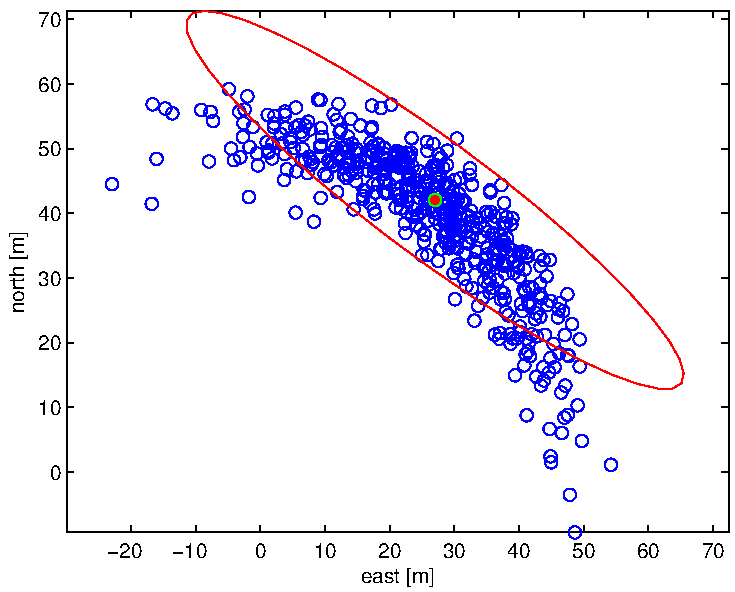
\includegraphics[width=0.45\linewidth]{fig/linear.pdf}} \\
	\subfigure[{\scriptsize UT sampled}]{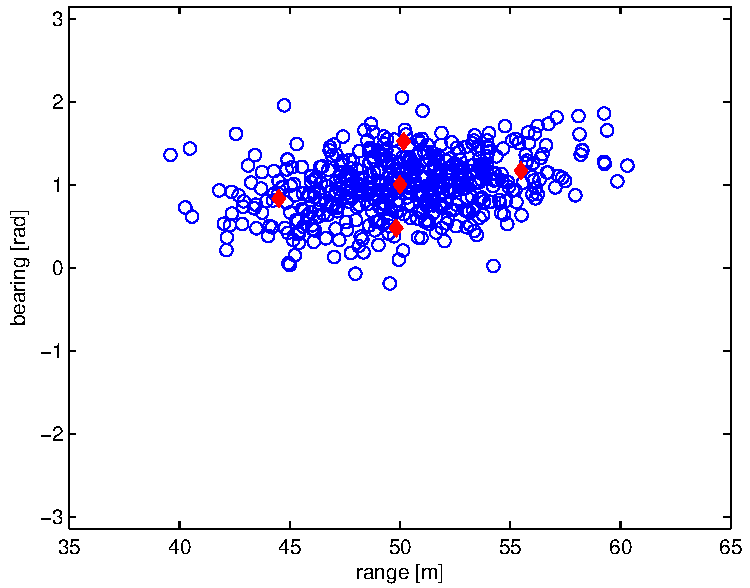
\includegraphics[width=0.45\linewidth]{fig/orig-samples.pdf}}
	\subfigure[{\scriptsize $\hat{X}, P$ (UKF)}]{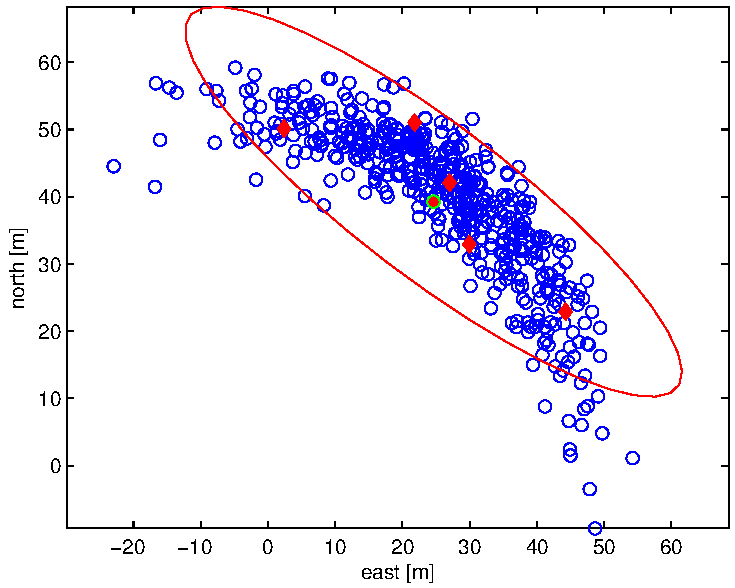
\includegraphics[width=0.45\linewidth]{fig/unscented.pdf}} \\
	\end{figure}
	\end{block} 

\column{.48\textwidth}
%\centering 
\vspace{-10pt}
\begin{columns}
\column{.38\textwidth}
\begin{block}{EKF}
{\scriptsize linearisation of the transform}
\end{block}
%\textbf{EKF} \\
%
\column{.58\textwidth}
\begin{block}{UKF}
{\scriptsize pdf is estimated using a collection of samples of a GRV propagated through the nonlinear transformation}
\end{block}
%\textbf{UKF} \\
%
\end{columns}
\vspace{5pt}
\textbf{Unscented Transform} (UT): selects the samples of a Gaussian and assigns a weight to each. 
	\begin{itemize}
		\item {\footnotesize guarantees $2^{nd}$ order Taylor expansion accuracy \cite{julier96}} 
		\item {\footnotesize no infamous Jacobians} 
		\item {\footnotesize same computational cost as EKF} 
	\end{itemize}	
\end{columns}
\end{frame}